\documentclass[10pt,a4paper]{article}
\usepackage{amsmath}
\usepackage{amsfonts}
\usepackage{amssymb}
\usepackage{natbib}
\usepackage{graphicx}
\usepackage[left=2cm,right=2cm,top=2cm,bottom=2cm]{geometry}
\usepackage{arydshln}

\title{Validating Plate Boundary Observatory borehole strainmeter data with GNSS derived strain} 
\author{Trever T. Hines and Eric A. Hetland}
\begin{document}

\maketitle


\section{Introduction}\label{sec:Introduction}
The Plate Boundary Observatory maintains 82 borehole strain meters (BSMs), most of which are installed along the Western United States. BSMs are able to detect geophysical processes such as coseismic and postseismic deformation \citep[e.g.,][]{Langbein2006,Langbein2015}, slow slip events \citep[e.g.,][]{Dragert2011}, and seismic wave propagation \citep{Barbour2017}. BSMs are intended for measuring deformation over timescales of minutes to months. At longer timescales, BSM data is contaminated by factors such as borehole relaxation \citep{Gladwin1987}. Slow slip events and postseismic deformation occur on timescales that near the upper limit of what BSMs can be expected to resolve. Another complication with BSM data is that the strain measured at the borehole may deviate from the regional strain due to local topographic or geologic features \citep{Berger1976}. Due to these sources of noise, it can be difficult to use BSM data quantitatively in, for example,  geophysical inverse problems.

In this study, we assess the ability of BSMs to measure strain resulting from slow slip events (SSEs) on the Cascadia subduction zone. This is done by comparing BSM data to strain derived from GNSS data. There are about forty BSMs in the Pacific Northwest and only five of them, B003, B004, B005, B007, and B018, record noticeable deformation from SSEs. Of these stations B005 and B007 are collocated. We show that only station B004 produces strain that is in reasonable agreement with GNSS derived strain rates.  Station B018 records shear strains with opposite polarity as the GNSS derived strains. This discrepancy can be explained by an $25^\circ$ error in the recorded orientation of the instrument. 

GNSS derived strains are computed with Gaussian process regression using the method described in \citep{Hines2017}.   

\section{Data}
Each of the PBO BSMs are Gladwin tensor strain meters, which contain four extensometers, or gauges, oriented $60^\circ$, $60^\circ$, and $30^\circ$ apart from each other. We denote the extension measured at gauge $i$ as $e_i$, and the strain tensor components as $\varepsilon_{xx}$, $\varepsilon_{yy}$, and $\varepsilon_{xy}$, where $x$ and $y$ indicate the east and north direction, respectively. The extensions measured at BSMs are traditionally converted into areal strain, $\varepsilon_a = \varepsilon_{xx} + \varepsilon_{yy}$, differential strain $\varepsilon_d = \varepsilon_{xx} - \varepsilon_{yy}$, and engineering shear strain, $\varepsilon_s = 2\varepsilon_{xy}$. Data from only three gauges are needed to estimate these strain components, and the PBO BSMs contain an extra gauge for redundancy. Using $\theta_0$ the denote the orientation of gauge 0, in degrees north of east, the strain components can be expressed in terms of the gauge measurements through the equation 
\begin{equation}\label{eq:GaugeToStrain}
\left[\begin{array}{c}
\varepsilon_a \\
\varepsilon_d \\
\varepsilon_s \\
\end{array}\right]
=
2\mathbf{K}^{-1}\left[\begin{array}{ccc}
1 & \cos(2\theta_0) & \sin(2\theta_0) \\
1 & \cos(2(\theta_0 + 60)) & \sin(2(\theta_0 + 60)) \\
1 & \cos(2(\theta_0 + 120)) & \sin(2(\theta_0 + 120)) \\
1 & \cos(2(\theta_0 + 150)) & \sin(2(\theta_0 + 150)) \\
\end{array}\right]^+
\left[\begin{array}{c}
e_0 \\
e_1 \\
e_2 \\
e_3 \\
\end{array}\right],
\end{equation} 
where ``$+$" indicates the Moore-Penrose pseudoinverse and $\mathbf{K}$ is a coupling matrix describing how instrument strains relate to the crustal strains \citep{Hart1996}. In this paper $\varepsilon_a$, $\varepsilon_d$, and $\varepsilon_s$ are ideally intended to represent crustal strains. We assume that BSMs are installed in homogeneous, isotropic rock, allowing us to write the coupling matrix as
\begin{equation}\label{eq:CouplingMatrix}
\mathbf{K} = 
\left[\begin{array}{ccc}
c & 0 & 0 \\
0 & d & 0 \\
0 & 0 & d \\
\end{array}\right],
\end{equation}  
where $c$, and $d$ are response factors that depend on the elastic properties of the instrument, the grout, and surrounding rock \citep{Gladwin1985}. Based on the analysis of \citet{Gladwin1985}, we use $c=1.5$ and $d=3.0$. UNAVCO, the organization responsible for maintaining the PBO BSMs and disseminating their data, use these same response factors for their final data products. 

Local topographic or geologic features can cause $\mathbf{K}$ to have non-zero off diagonal elements. If possible, the components of $\mathbf{K}$ should be determined in-situ by calibrating the BSM data with a well known strain source, such as diurnal and semi-diurnal tides \citep{Hart1996,Roeloffs2010,Hodgkinson2013}. \citet{Hart1996} calibrated a BSM at Pinyon Flat, using the tidal strains recorded at a collocated laser strain meter. This calibration method is, of course, not possible for most PBO BSMs. \citet{Roeloffs2010} and \citet{Hodgkinson2013} calibrated PBO BSMs using theoretical predictions of tidal strains \citep[e.g.,][]{Agnew1997}. This approach is still not adequate for BSMs near large local bodies of water, which can make it difficult to form an accurate theoretical estimate of tidal strains. As determined by \citet{Roeloffs2010}, the five BSM stations considered in this paper are too close to the Straight of Juan de Fuca to be accurately calibrated with tidal strains. Since in-situ calibration is not possible, we acknowledge that our choice for $\mathbf{K}$ is likely to be a significant source of error in BSM data. Another potential source of error is the assumed orientation for $\theta_0$. This orientation is determined by a compass on the instrument, and it is possible that magnetic minerals in the surrounding rock can give the compass an erroneous reading. 

that record extension along four azimuths  
In this study we use the level2 PBO BSM data provided by UNAVCO at www.unavco.org.     


\section{Method}\label{sec:Method}
bar
\begin{figure}
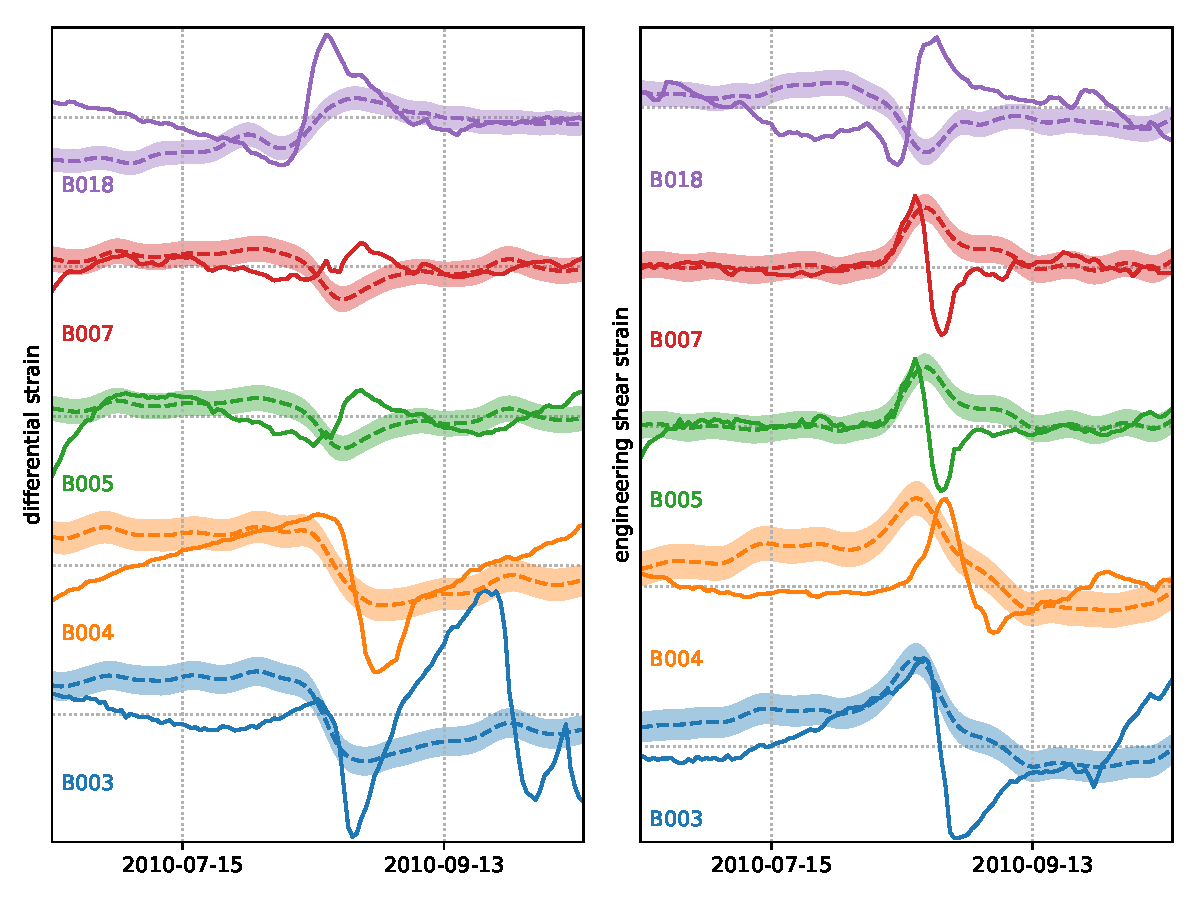
\includegraphics[scale=0.8]{figures/Figure_1}
\caption{foo}   
\label{fig:Demo1}
\end{figure}

\bibliographystyle{apalike}
\bibliography{mybib}  
 
\end{document}